% Created 2022-08-29 Mon 20:12
% Intended LaTeX compiler: pdflatex
\documentclass[11pt]{article}
\usepackage[utf8]{inputenc}
\usepackage[T1]{fontenc}
\usepackage{graphicx}
\usepackage{longtable}
\usepackage{wrapfig}
\usepackage{rotating}
\usepackage[normalem]{ulem}
\usepackage{amsmath}
\usepackage{amssymb}
\usepackage{capt-of}
\usepackage{hyperref}
\documentclass[11pt]{article}
\usepackage[margin=.7in, top=1.2in]{geometry}\usepackage{fancyhdr}\pagestyle{fancy}\fancyhf{}\lhead{Public Transportation Systems}\rhead{Notes}\rfoot{\thepage}\
\usepackage{enumitem}
\setlist{\setlength\itemsep{0em}\setlength\topsep{0em}}}
\author{Alex Bellon}
\date{\today}
\title{}
\hypersetup{
 pdfauthor={Alex Bellon},
 pdftitle={},
 pdfkeywords={},
 pdfsubject={},
 pdfcreator={Emacs 28.1 (Org mode 9.6)}, 
 pdflang={English}}
\begin{document}

\tableofcontents

\clearpage
\section{Introduction}
\label{sec:org83bb1eb}

\subsection{Transit right now}
\label{sec:orgcca62f0}
\begin{itemize}
\item Ridership is increasing, but small
\item Strong financial support from
\item Trends in modal split
\begin{itemize}
\item Auto is above 80\%
\item Transit 2-3\%
\item Biking and walking are the same as transit
\end{itemize}
\end{itemize}

\subsection{Funding}
\label{sec:org06d0ae5}
\begin{itemize}
\item In North America, it's divided into captial and operating expenses
\item Fares only pay \textasciitilde{}1/3 of operational expenses
\item Lots of federal support for capital expenses - almost 40\%
\begin{itemize}
\item Since operating expenses are funded less, this encourages more building and less maintenance
\end{itemize}
\item Fuel taxes in NA are 10-20\% of what they are in Europe
\end{itemize}

\subsection{Traditional Arguments Supporting Transit}
\label{sec:orgb742311}
\begin{itemize}
\item Equity: travel for those who can't drive
\item Congestion
\begin{itemize}
\item Not such a good argument, papers don't support it. The capacity released it quickly filled again
\end{itemize}
\item Better for the environment
\begin{itemize}
\item Actually, effort it better spent making cars cleaner since they're like 80\% of transport
\end{itemize}
\end{itemize}

\subsection{Critical assessment}
\label{sec:orgb8a83b0}
\begin{itemize}
\item Transport has been stabilized
\item Success stories (NYC, Houston(?), Seattle)
\item Institutional changes are occurring slowly
\end{itemize}

\subsection{Future influences}
\label{sec:org6b8653c}
\begin{itemize}
\item Urban form
\item More old people
\item Better tech to improve performance
\item Public has higher expectation (you know exactly when the bus is coming)
\end{itemize}

\subsection{Ingredients for future success}
\label{sec:org041ea10}
\begin{itemize}
\item Maintain supportive coalition
\item Expand the definition of public transport
\item Greater private sector involvement
\item Aggressive implementation of new technology
\end{itemize}

\clearpage
\section{Data Collection Techniques and Program Design}
\label{sec:orgffe74e1}

\subsection{Summary of current practice}
\label{sec:org5be6c7e}
\begin{itemize}
\item Used to be manual
\item Now is collected with IoT devices
\item \textbf{Automated Data Collection Systems (ADCS)}
\begin{itemize}
\item \textbf{Automated Fare Collection Systems (AFC)}
\begin{itemize}
\item Tapping your card on/off the vehicle
\end{itemize}
\item \textbf{Automatic Vehicle Location Systems (AVL)}
\begin{itemize}
\item GPS tracking for buses, train tracking based on circuit occupancy
\end{itemize}
\item \textbf{Automatic Passenger Counting Systems (APC)}
\begin{itemize}
\item Sensors in bus doors
\begin{itemize}
\item Use break beam sensors to tell if you're getting on or off (out of 2 beams which do you break first)
\end{itemize}
\item Counts from fare barriers
\item Load weight calculators on trains
\begin{itemize}
\item In trains the brakes apply force proportional to the load in each car (lighter cars need less braking, heavier cars need more, so they dont run into each other)
\end{itemize}
\end{itemize}
\end{itemize}
\end{itemize}

\subsection{Passenger counting techniques}
\label{sec:orgea52cec}
\begin{itemize}
\item Manual - checker (a person)
\begin{itemize}
\item Ride check (on the bus, on/off counts and running time)
\item Point check (load on board, headway - time between buses)
\end{itemize}
\end{itemize}

\subsection{Sampling}
\label{sec:org02bc3f1}
\begin{itemize}
\item \textbf{Simple random sampling}
\item \textbf{Systematic sampling} - every 6 days, etc
\item \textbf{Cluster sampling} - do as much data collection as possible
\item \textbf{Ratio estimation/Conversion factors}
\item \textbf{Stratified sampling} - sample sizes for each thing separately
\begin{itemize}
\item E.g. you want information about students: get a large sample size on routes that serve universities
\end{itemize}
\end{itemize}

\subsection{Tolerance and confidence level}
\label{sec:org66d4445}
\begin{itemize}
\item Accuracy has 2 dimensions
\begin{itemize}
\item Relative tolerance: \(\pm 10\%\)
\item Absolute tolerance: \(\pm 3.3\)
\end{itemize}
\end{itemize}

\clearpage
\section{Modal Characteristics and Roles}
\label{sec:orgbad3847}

\subsection{Spectrum of services}
\label{sec:orge3d3437}
\begin{center}
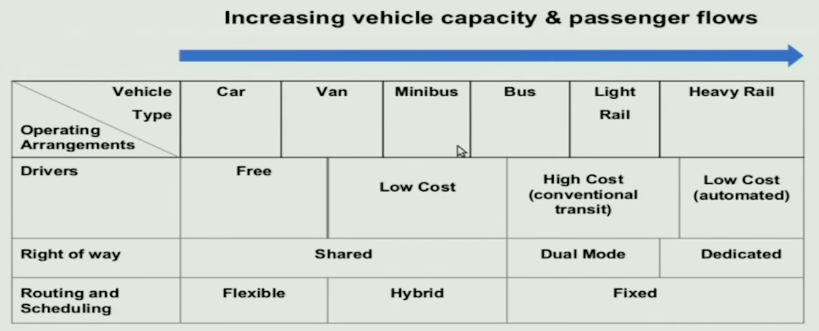
\includegraphics[width=.9\linewidth]{.images/modes.png}
\end{center}

\subsection{Transit categories}
\label{sec:org5c80216}
\begin{itemize}
\item Rights of way - degree of separation
\begin{itemize}
\item Surface with mixed traffic (light rail/buses)
\item Longitudinal separation by at grade crossing (light rail/bus rapid transit)
\item Full separation (at grade/tunnel/elevated)
\end{itemize}
\item Technologies
\begin{itemize}
\item Support (how they contact the groups)
\begin{itemize}
\item Rubber tire on concrete (cars, buses, some rail like Paris Metro)
\item Steel wheel on steel rail
\item Maglev
\item Suspended cars
\item Water
\item Others
\end{itemize}
\item Guidance (lateral control)
\begin{itemize}
\item Steered by driver
\item Guided by track
\item Others
\end{itemize}
\item Energy and propulsion
\begin{itemize}
\item Combustion engine
\item Electric
\item Compressed natural gas (CNG)
\item Hybrid
\item Others
\end{itemize}
\item Control (longitudinal)
\begin{itemize}
\item Manual/visual
\item Manual/signal
\item Automatic
\end{itemize}
\end{itemize}
\end{itemize}

\subsection{Basics of train control}
\label{sec:org42e4570}
\begin{itemize}
\item Divide the system into blocks
\begin{itemize}
\item If a train is occupying a section, do not let any trains in the section immediately before
\item For each block further, slowly increase speed limit in that block from nothing (0, 10, 25, 40,\ldots{})
\end{itemize}
\item Block system constrains the frequency of service
\item Moving block system increases capacity, usually used with automatic driving systems
\end{itemize}

\subsection{Levels of automated protection}
\label{sec:org43cce73}
\begin{itemize}
\item None - advisory way signals
\item Manual setting of speed below speed limit - train will be automatically braked if over speed limit
\item Automatic train supervision/regulation
\item Full automation - sometimes has operators, needs to have platform screen doors to keep people off of track
\item Capacity increased through moving block or communication based train control
\end{itemize}

\subsection{What is a bus?}
\label{sec:orga3b5f38}
\begin{itemize}
\item Vehicle size - 10-250 passengers
\item Floor height (high floor/low floor)
\begin{itemize}
\item Low floor is better for accessibility, has lower dwell time
\end{itemize}
\item Right of way - all options available
\item Guidance - often manual, sometimes systems
\item Propulsion - all options available
\item Fare payment - pay outside, or pay in the bus
\end{itemize}

\subsection{Examples of bus systems}
\label{sec:orgf8cbb5c}
\begin{itemize}
\item Bi-articulated buses are a thing
\item In Curitiba, bi-articulated buses have high floors, and have to be boarded at specific stations with fare gates
\item The Cambridgeshire Guided Busway has buses operating on dedicated ``tracks'' of pavement
\begin{center}
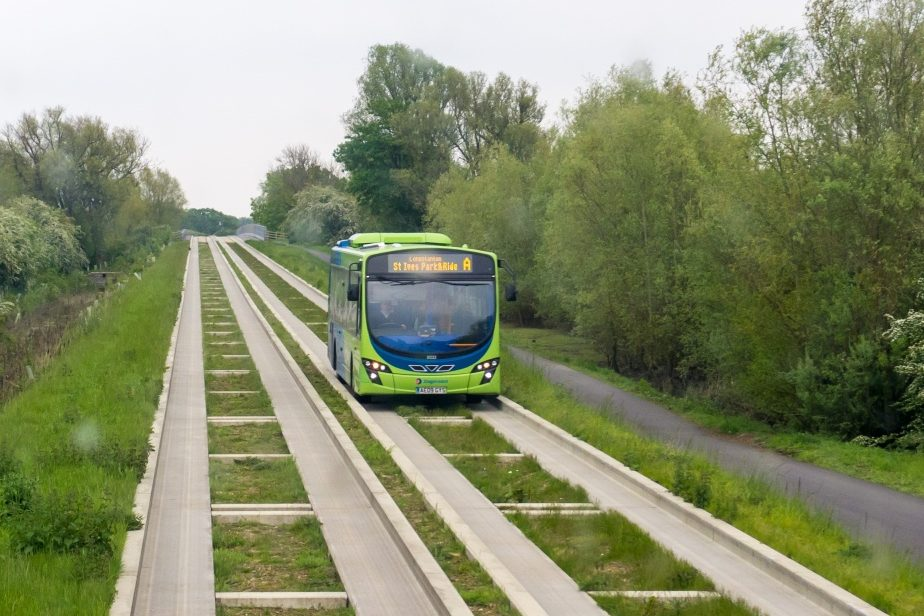
\includegraphics[width=.9\linewidth]{.images/busway.jpg}
\end{center}
\begin{itemize}
\item Buses can also be \href{https://en.wikipedia.org/wiki/Guided\_bus\#Optical\_guidance}{optically guided}, following a line on the floor with a camera
\end{itemize}
\end{itemize}

\subsection{Light Rail}
\label{sec:org50e730f}
\begin{itemize}
\item Vehicle design
\begin{itemize}
\item High/low floor
\item Articulated or not
\end{itemize}
\item Right of way
\begin{itemize}
\item All options available
\end{itemize}
\item Operation
\begin{itemize}
\item Automated or manual
\end{itemize}
\item Power
\begin{itemize}
\item Overhead catenaries
\item Third rail
\begin{itemize}
\item On street rails, the third rail is electronically controlled and is only powered when the train is coming
\end{itemize}
\end{itemize}
\end{itemize}

\subsection{Heavy Rail}
\label{sec:org2df6156}
\begin{itemize}
\item Length
\begin{itemize}
\item Limited by station length
\item In some cases (like in London) they allow the last door of the last car to stay in the runnel
\end{itemize}
\item Turning radius
\item Right of way
\begin{itemize}
\item At-grade
\item Elevated
\item Tunnel
\end{itemize}
\item Station spacing
\item Control
\item Power
\end{itemize}

\subsection{Commuter Rail}
\label{sec:orgdb0d060}
\begin{itemize}
\item Vehicles operating in trains with long station spacing
\item Fare collection strategies
\item Line length
\item Through routing in CBD [central business district] (cross through city or go there and back)
\begin{itemize}
\item Where to put trains when you're done
\end{itemize}
\item Station spacing
\item Parking capacity
\end{itemize}

\subsection{Traditional and new service concepts}
\label{sec:org932a5f1}
\begin{itemize}
\item Traditional
\begin{itemize}
\item Bus on shared right of way
\item Streetcar on shared right of way
\item Heavy rail on exclusive ROW
\item Commuter/regional rail on semi-exclusive ROW
\end{itemize}
\item New
\begin{itemize}
\item Bus rapid transit
\item Light rail on exclusive ROW
\end{itemize}
\end{itemize}

\subsection{Increasing diversity}
\label{sec:org8c7d3cb}
\begin{itemize}
\item Driver arrangements
\begin{itemize}
\item Part timers (cover peaks), 10 hour day (to cover peaks that are 8 hours apart), payment by vehicle type
\end{itemize}
\item Routing and scheduling
\item Vehicle types
\item control options
\item Priority options
\item Dual mode operation
\end{itemize}

\subsection{Bus vs rail comparison}
\label{sec:org19bd4ca}
\begin{itemize}
\item Rail advantages
\begin{itemize}
\item Higher capacity
\item Lower unit operating cost
\item Better service quality
\item Stronger land use influence
\item Fewer negative externalities
\end{itemize}
\item Bus advantages
\begin{itemize}
\item Low capital costs
\item Wide network coverage
\item Single vehicle trips
\item Flexibility
\item Dual mode nature
\end{itemize}
\end{itemize}

\section{Short Range Planning}
\label{sec:org15b9dd8}

\subsection{Public transit planning}
\label{sec:org1cff55d}
\begin{itemize}
\item Long range (>3 years)
\begin{itemize}
\item Major capital investments, infrastructure
\item Usually in collaboration with government
\end{itemize}
\item Medium range (1-3 years)
\begin{itemize}
\item Fleet size, network size, fare policy
\item Usually in collaboration with government
\end{itemize}
\item Short range (<1 year)
\begin{itemize}
\item Route structure, service frequency
\item Incremental changes
\item Can be handled only by the transit authority
\end{itemize}
\item Control (real time)
\begin{itemize}
\item Revise schedule and route of specific vehicle
\end{itemize}
\end{itemize}

\subsection{Operational planning process}
\label{sec:orgfa3aa42}
\begin{itemize}
\item Right of way + demand => bus route design => routes and stops
\item Service + demand => set timetables => departure times
\item Travel time constraints => scheduling vehicles => vehicle schedules
\item Operator and union constraints => scheduling drivers => crew schedules
\end{itemize}

\subsection{Transit service guidelines}
\label{sec:orgd0bca7b}
\begin{itemize}
\item Goals => objective => measures => standards
\item Early arrivals are not considered on time, because it may still cause people to miss connections
\item Purpose
\begin{itemize}
\item Communicate to the public and their representatives how decisions are made on changes in the transit network and the allocation of resources
\item Ensure acceptable level of service quality
\item Provide a consistent and fair bases for
\begin{itemize}
\item Evaluating existing services
\item Considering new services
\end{itemize}
\item Balance impreovements with efficient use of resources
\end{itemize}
\end{itemize}

\subsection{Aspects covered by service guidelines}
\label{sec:org64f066a}
\begin{itemize}
\item Service design
\begin{itemize}
\item Factors that are important to riders:
\begin{itemize}
\item Frequency
\item Waiting time
\item Reliability
\item Access
\end{itemize}
\item Why are frequency and waiting time both here?
\begin{itemize}
\item Waiting time can be independent of waiting time - if a bus comes early, it will change waiting time
\end{itemize}
\end{itemize}
\item Operating perfornace
\begin{itemize}
\item Service quality
\end{itemize}
\end{itemize}

\subsection{Service design: schedule}
\label{sec:org6c74d67}
\begin{itemize}
\item Two main components
\begin{itemize}
\item Maximum (policy) headways
\item Maximum passenger crowding
\begin{itemize}
\item Usually for peak corridors
\end{itemize}
\end{itemize}
\end{itemize}

\section{Short Range Planning, con't.}
\label{sec:orga189e82}

\subsection{Service reliability}
\label{sec:orga75d05b}
\begin{itemize}
\item Walk up service
\begin{itemize}
\item Schedule free
\item Headway-based, <10 minutes
\item Performance based on headway
\end{itemize}
\item Scheduled service
\begin{itemize}
\item >= 10 minute headway
\item Performance measurement based on punctuality
\end{itemize}
\end{itemize}

\subsection{Alternative benefit measures}
\label{sec:orgfa3ab22}
\begin{itemize}
\item Revenue
\begin{itemize}
\item Relevant to financial concerns and willingness to pay, discounts reduced fare trips and favors higher income passengers
\end{itemize}
\item Passengers
\begin{itemize}
\item Reflects number of people who benefit, values each passenger equally, but doesn't reflect trup length or linked trips
\end{itemize}
\item Passenger miles
\begin{itemize}
\item Weights longer trips more, but hardest to measure since most systems don't have an exit
\end{itemize}
\item Net cost
\begin{itemize}
\item Usually most directly constrained, but hardest to estimate (if you're planning a new service, you won't know revenue)
\end{itemize}
\item Cost
\begin{itemize}
\item Also directly constrained, but hard to estimate
\end{itemize}
\item Vehicle miles
\begin{itemize}
\item Easy to measure, only reflects \textasciitilde{}30\% of bus costs and penalized fast service
\end{itemize}
\item Vehicle hours
\begin{itemize}
\item Easy to measure, related to >50\% bus costs, but doesn't reflect cost differences between peak and off-peak
\end{itemize}
\end{itemize}
\end{document}
